% !Mode:: "TeX:UTF-8" 

\BiChapter{相关工作综述}{pdpintro}
\label{sec:pdpintro}



%重要概念介绍

%重要技术的介绍

%研究的基石

%研究的关键问题



%目标,软件功能硬件卸载,提速。在硬件中增加可编程逻辑的对外性能。


\BiSection{本章引论}{}
本章综述了国内外网络基础设施技术的演进,主要分析其主要技术特征和局限短板,重点关注了现阶段实际情况下SDN可编程数据平面的灵活性与性能矛盾点,为本文研究工作指明了方向和意义所在。







\BiSection{网络可编程的发展历程}{}
%研究领域发展趋势介绍





\BiSubsection{软件实现---早期网络基础设施}{} %IP10k https://mp.weixin.qq.com/s/1tUXilmvbIzlMoDQUuC2Jg 《可编程数据平面调研_说的还不错.pdf》

%主旨:过去软件的好处,软件的坏处,现在软件的好处,软件的坏处

网络对于业务的基本价值是网络实现了数据在计算机之间的任意传输。在早期\footnote{上世纪90年代中期以前},由于用户数量、计算机算力、存储、硬件性能都过于微弱,作为连接所有终端、服务与用户的管道,网络的主要特点集中在连通性、可行性和初期探索性上。在一个简单的星型拓扑中,一个路由器其实就是一台普通计算机。在学术和产业界的初期,人们并没有意识到网络需要单独拎出使其成为一套独立系统的价值。这在侧面也体现出软件作为网络实施载体的特点:“灵活性”。即:对于处理并实现一个新兴事物,软件可以发挥其巨大的灵活性优势,使其可以作为一种为数不多的手段,快速实现工程师学者的任意的新的思想。

后期随着社会生活、技术进步,步入信息时代之后逐渐发现人与人之间数字信息交互的需求和价值越来越大。因而研究重点开始关注在如何实现快速的包交换、路由查找。为此人们开始提出各种快速交换的数据结构:Cache优化、哈希表、Radix Tree(树查找)等。很长时间基于软件的转发设备核心架构都没有变化,唯一变化的是跟随摩尔定律成长的芯片技术。CPU和存储每18月性能翻番,网络设备的性能也顺势而上,人们对网络的发展信心十足。网络处理从单CPU向多CPU并行,向分布式存储cache结构进行了小小扩展,但也好像失去了创新的动力。然而人们对信息量需求的增长却大大快于摩尔定律。到2011年底,我国互联网入户带宽平均接近20Mbps\citeup{20112m}。从最初14.4Kb的拨号上网,网络容量的发展几乎是以每18个月翻10倍的速度在增长。在数百兆的路由性能要求下用软件作为转发设备基础比较合适,但如果核心网要升级到1G或数十G以上更高的带宽就会面临技术、成本等多方面的瓶颈。

\BiSubsection{向硬件过渡}{} %IP10k

数据包交换对于CPU来讲是一种很累的工作。虽然数据包转发算法既简单、又高效,但面对无穷无尽的任务量,依靠指令集的软件转发架构存在访存效率差、CPU无法批处理等劣势。这时研究人员抛弃了基于指令集的软件架构,开始思考基于专用硬件电路(Application-specific integrated circuit, ASIC)的数据包处理模型。此时硬件转发的发展目标是如何增大交换设备的交换容量、以及研究具有更好的可扩展性的设计方案。电路交换Crossbar(交叉开关)\citeup{mckeown1997fast}架构追求$N$队列输入到$N$队列输出的无阻碍转发,其思想的本质是使用一种二维电子开关(Switching)矩阵来增强交换设备的转发能力。矩阵中有$N^2$个开关交点,可以实现任意的$N_i$输入映射到$N_j$输出,也易实现多对一、一对多映射。因报文长度不固定开关数量大导致控制器硬件算法难度高\citeup{katevenis2004variable,aybay2000method},以及传输冲突等问题\citeup{nachiondo2009buffer},此后的一系列技术创新集中在如何降低Crossbar的管理时延、提高理论吞吐容量\citeup{cisco12000seriesrouters,yoshigoe2001parallel}。人们也在思索如何在扩展交换容量时节约芯片面积,其中重要的思想是由单模块交叉开关联结为多交叉开关结成的网(fabric)\citeup{heitner2004folded}。有专用硬件电路的加持,业界把单芯片交换能力提升至25.6Tbps\citeup{broadcom256t}。能够支持在一个大规模数据中心内可以支持256台配置有100G网的卡服务器形成一个小区进行高速互联,这样的组网计算机的并行处理能力已经足够一个通常规模大数据算法使用。单芯片容量升高会使晶体管面积成$O(N^2)$规模增长从而变得不再划算。如果想支持1024台服务器,网络架构商可以选用两级Spine\&Leaf(骨干与边缘)架构,使用12\footnote{12=4(Spine)+8(leaf),每个leaf节点对外暴露一半的接口容量,最终扩展4倍到达102.4Tbps}块25.6Tbps的交换芯片组成一个102.4Tbps的扩展规模网络。

当设备被大规模组网时,网络的管理问题变得尖锐。早期互联网的发展非常迅速,因为设备的扩展就是简单对接,每个设备独立控制自己,具备对外扩展的策略。随着时间的流逝,网络内产生了成百上千个新IETF RFC(网络工程备忘录)和IEEE标准。设备制造商需要用同一个产品向各类运营商提供服务,这导致在同一款路由设备产品中堆叠的功能特性也越来越多。一些ISP路由设备的源代码甚至超过1亿行,是最复杂电话交换机的10倍以上,要知道电话交换机也曾需要支持上百种协议\citeup{ethane},即使大多数客户只需要其中某一种功能。互联网也为这种高复杂度付出了代价:设备臃肿部件数量庞大、不节能效率低下、价格昂贵、API的设计随意。由于路由设备行业门槛较高,初创企业难以进入市场并发挥创新能力。此时大的路由器供应商也为路由器的可靠性、高复杂性、安全性等问题苦恼,网络的创新速度又变慢了。

%TODO:网络管理是传统的,过去小规模是有优势的,但当规模大了之后收敛慢,编程复杂,可以参考ethan论文 -> From Ethane to SDN and Beyond,然后主要找传统网络的劣势



\BiSubsection{软件定义网络演进---软、硬任务划分,物理隔离}{} %http://blog.sina.com.cn/s/blog_13743c4140102vh7e.html openflow 标准演进过程 
%《软件定义网络 SDN 数据平面带状态转发》 page14
%《阿里巴巴)page10 12

%先说问题,

%再说SDN的解法
1)数据平面的统一化与精简控制软件。

软件定义网络(Software Defined Networking,SDN)\citeup{mckeown2008openflow}的概念赋予运营商集中式或半集中式程序控制的便利。网络设备控制面和数据面的物理隔离,给这种体系架构带来经济学层面的优势:能将复杂的数据平面管理功能软件集中在少数几个地方,具有统一设计的数据平面抽象。最开始人们发现,每一个运行在网络系统里的数以千计的交换机和路由器都运行着一个程序处理器。大量这种分布式控制设备的数据平面运行的软件其实是一样的,但却需要设备数量十分之一\citeup{casado2007ethane}的网络管理员去不停地确保网络正常运转。相比于运维效率低,不确定性才是最危险的。由于传统网络的控制平面是分布式的,在正常运行状态下没有人能够有一个清新的网络运行图,因而在网络出现问题时管理人员很难调试。对于数据平面的设计思想也很直接,数据平面必然完全接受控制平面的控制策略,而数据平面输入输出都是数据报文,那么数据平面内的所有操作都可以由Matching--Action(匹配---执行)模型抽象出来。网络的功能就由远端控制平面上的软件来定义,这将有助于网络的“创新力”。因为网络功能、协议的定义不再只能由设备供应商提供,而能够由真正维护和使用网络的操作人员现场定义/修改。同时,操作人员能够拥有网络全局视图,对保障网络运行和安全控制也有极大的促进。

数据平面与控制平面之间的交互称为“南向接口”,目前南向接口的事实标准是2008年由斯坦福大学提出的OpenFlow协议。OpenFlow协议由最开始的OpenFlow1.0,快速发展到现在的OpenFlow1.6。几年时间,OpenFlow协议已经逐步完善到网络的各个细分领域:流量调度\citeup{al2010hedera,heller2010elastictree},光适配\citeup{openflowoptical},广域网\citeup{jain2013b4,aryakasdwan},超转发\footnote{Super Packet Transport Network,~SPTN。一种硬件功能组件可分解的高效可编程网络框架。}\citeup{openflowsptn}等。

2)云和虚拟交换。
%ip1w

随着云计算的持续发力,虚拟化成为其中重要技术。虚拟机内部互相通信需求增高,基于SDN的OpenVSwitch同样也令虚拟交换机编程更容易、转发更方便。软件定义网络加速云虚拟化的创新,软件定义网络能够提供非常复杂的虚拟网络语义,支持快速迭代。数据中心网络性能的提升需求远远快于CPU的处理能力的增长,通常来讲,CPU一个核心能够支持10Gpbs的转发性能。对于未来数据中心服务器百G带宽需求,也许需要消耗CPU总体性能的20\%\footnote{以常见Intel志强48核心CPU处理器为例。}。


\BiSubsection{协议无关数据平面可编程演进---可编程性层次划分,逻辑隔离}{} %《可编程数据平面调研_说的还不错.pdf》

%《软件定义网络关键技术及相关问题的研究》 page10


%然而如今众多快速出现的功能,并不是一个固定域就能分类完成。
1)扩充报文编码与设备快速更新

如果说SDN给出了控制层的全局视野,那么这种协议无关可编程的数据平面给出了设备层的全局视野。SDN已经将数据平面高度抽象,操作人员可以灵活的定义什么样的流,以及对这种流进行怎样的操作。但是在数据平面内数据包头的匹配域却是预先规划好的。固有转发平面的设计思想会引起如下两个问题:其一,添加新特性需要跟业界讨论、以及等待很长的设备研发时间;其二,在数据平面内固化现实中可能出现的每一个网络协议字段造成宝贵计算资源的巨大浪费。满足新阶段的网络创新需要比SDN更好的灵活性、动态性。因此斯坦福大学提出了P4\citeup{p4}编程语言框架,这种语言有能力重新定义数据平面的包解析模式。P4源代码通过前端编译器编译为中间表示层代码,这个编译过程将提出源代码中的语义逻辑。之后需要根据不同的目标器件再进行后端编译,这个过程最终会生成目标器件对应的机器码,硬件可直接读取。目前P4的目标设备已经有基于ASIC的交换芯片、CPU、GPU和FPGA等多种实现。

P4是与流表式编程不同,它是另外一种维度的高层次可编程概念。在P4框架中,网络操作者可以根据新的设计,创造性地自行设计一种结构的数据包头字段。通过P4源代码,将新的包头结构编译到数据平面形成新的指令。这就实现了灵活定义数据平面解析过程。
P4的目标是让已经部署的硬件网络设备数据平面实现软件定义升级,可以达到在线无插拔地更换新设备的效果。P4的出现也首次实现了数据平面不同逻辑层面上的可编程性。

2)可编程硬件的未来

数据平面可编程概念引发了众多新技术和为解决不同问题所提出的创新实践,如图\ref{pdphistory},本文从不同方向架构梳理这些工作。

\begin{figure}[!ht]
	\centering
	
\includegraphics[scale=1]{pdphistory.pdf}
	\caption{可编程数据平面各界发展历史} \label{pdphistory}
\end{figure}

当设备处理接收进来的每个数据包时,数据平面是网络当中最关键的环节。通常需要用到专用的硬件设施,或者经过复杂优化后的软件加速方案。在硬件方面,数据平面可以在ASIC\citeup{de2009plug,anwer2010switchblade,intelflexpipe,rmt,tofino,tofino2},FPGA\citeup{naous2008implementing,yabe2011openflow,netfpga2014,han2015blueswitch,li2016clicknp,wang2017p4fpga,sdnet,firestone2018azure}, 网络处理器\citeup{intelixp4xx,xpliant,netronome},外挂有三态内容地址查找器件(TCAM\footnote{Ternary Content Addressable Memory,~TCAM})的系统\citeup{pagiamtzis2006content},在软件方面有基于快速包分类算法\citeup{feldman2000tradeoffs,kogan2014sax,srinivasan1999packet}的在CPU系统上实现\citeup{greenhalgh2009flow,lincswitch,indigo,cpqd,snabbswitch,ovs,molnar2016dataplane,pisces,panda2016netbricks,p42018behavioral,sonic,dalton2018andromeda}。从2008年提出软件定义网络,由于真实环境性能的需求,业界从未间断地开发基于硬件的可编程数据平面。在P4概念提出来之前,也有类似于半P4的混合型可编程数据平面,受限于设计架构,他们对于短长度域可以实现任意匹配,基本可实现常见协议的数据平面编程,但不能够有效支持宽域\citeup{de2009plug}。

由于硬件可编程技术的加持,外加比虚拟机更轻量级的容器、高速分布式存储、无服务架构、AI对I/O响应速度的要求,使得网络体系架构设计发展繁荣、爆炸增加。相信在未来业界将会出现更多的应用场景,这些场景也将会不断催生出功能更强大的可编程网络、以及更强大的性能。




\BiSection{网络可编程性的“图灵完备”}{}
%完备性与硬件平台的设计思路息息相关。https://www.zhihu.com/question/20115374 知乎问题解答



\BiSubsection{通用可编程性和可编程网卡}{}%虽说FPGA足够灵活,但卸载东西还是有难度
%NP
%1)介绍可编程网卡是什么
%2)介绍通用可编程性
%3)分析现阶段

上一章提到,我们需要使用智能网卡来卸载操作系统内的网络功能,以期望获得比CPU更好的效能,同时还可以兼顾网络设计中不断变化的革新需求。智能网卡也叫做可编程网卡,相比于普通网卡,一种认知认为\citeup{shinde2013we}:智能网卡不但可以完成网卡最基本的作用(主机与网络间通信),还应该有如下特征:输入输出多队列、TCP卸载、流量整形、规则过滤、虚拟化等。从而增强一些通用场景下的网络性能:带宽扩容、优化QoS\footnote{Quality of Service (QoS),服务质量}、降低CPU利用率、降低通信时延等。
%这只是一个下放了的交换机,说明我们掌握了网络数据通路内的控制面。
%已经跟不上形势了,1.ASIC功能固定,时间长,2.新的应用私人订制例如随路计算
如图\ref{asicsmartnic},是一个典型的ASIC智能网卡通路,易见,网卡将各种网络处理过程(流分类、流量工程、协议)硬化到专用硬件逻辑上,使处理效能增加。不难发现,基于ASIC的智能网卡本质类似于一个操作系统的外挂交换机,只是他与主机侧链接的延迟更短,主机拥有其完整的控制平面管理能力。

\begin{figure}[!ht]
	\centering
	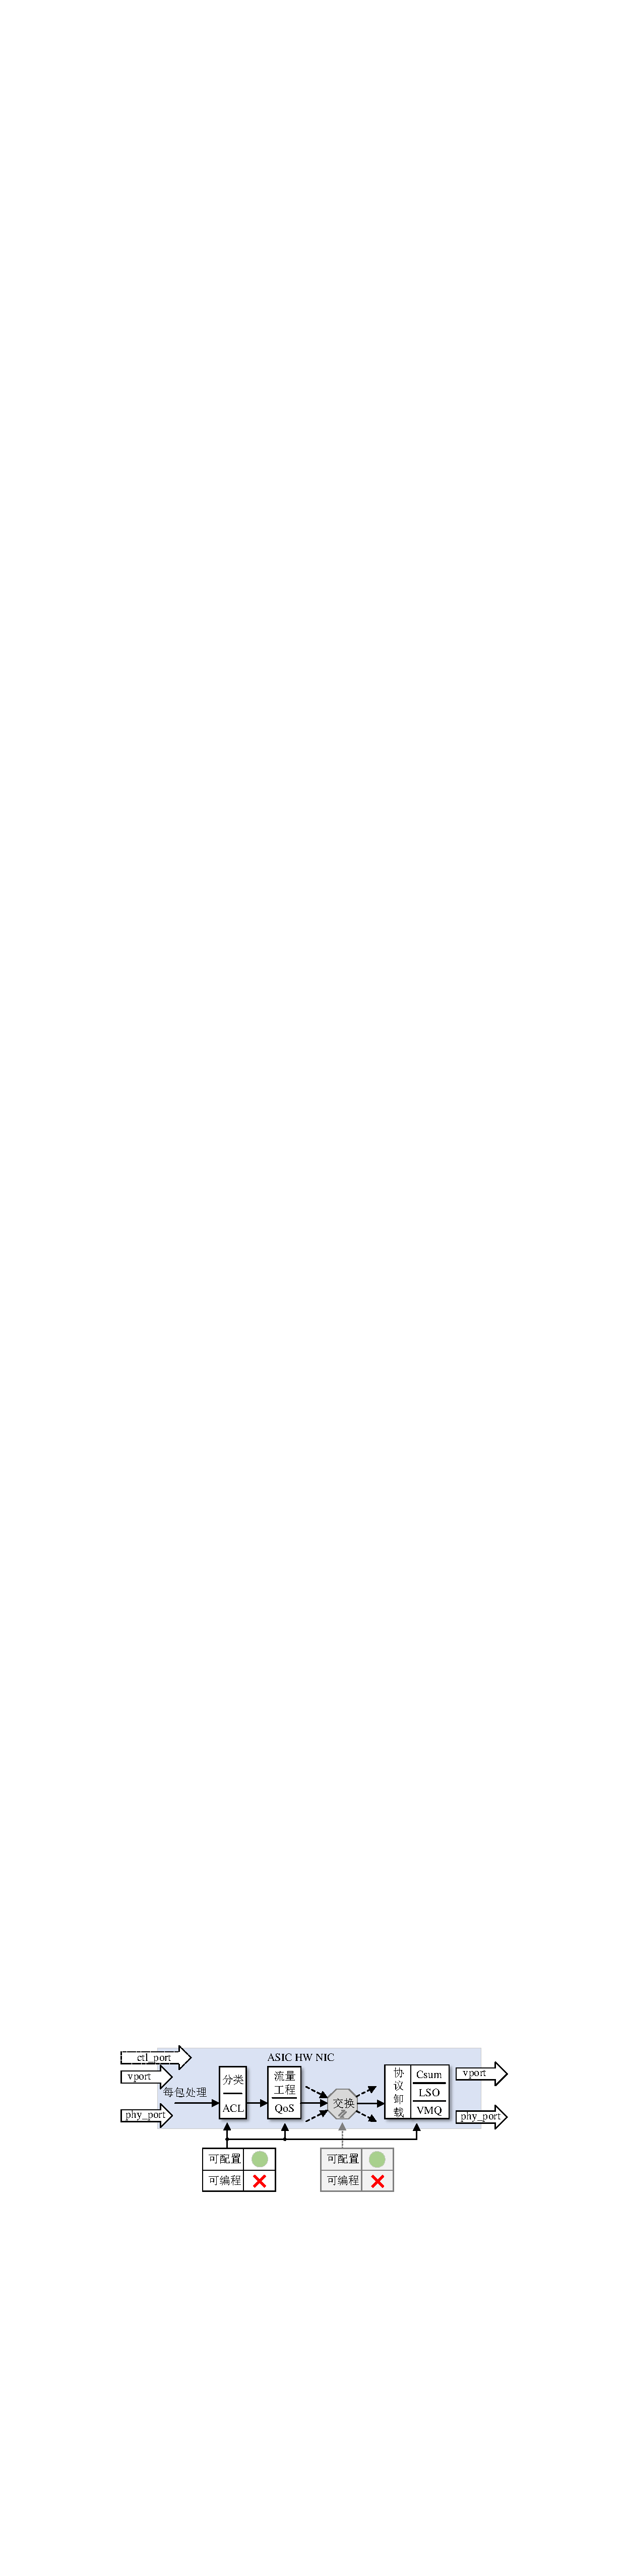
\includegraphics[scale=1]{asicsmartnic.pdf}
	\caption{基于ASIC的智能网卡架构} \label{asicsmartnic}
\end{figure}

这种开放控制平面的网卡架构,还称不上真正的智能网卡,因为它无法提供“核心部件”和“辅助部件”两方面的客制化的编程能力。首先,网卡的核心功能是一个数据包交换结构,完成“匹配---执行”操作,然而基于ASIC的网卡芯片出厂后就无法修改包头域的设置,核心部件不能实现可配置的交换,因而无法满足新协议的处理需求。第二,流水线中包括基于硬件电路的QoS、访问控制(ACL)、协议卸载等辅助部件。这些卸载功能如果无法支持新的网络协议栈,那么此类功能只能从网卡重新回到通用CPU中处理,几乎失去智能网卡的性能优势。ASIC的研发周期一般都比较久,并不能很好的适应目前快速迭代的网络架构需求,是缺乏适应性和可扩展性的。

随着时间的推移,人们还发现如果能够将计算\citeup{costa2012camdoop,sapio2017network}、随路功能聚合\citeup{mai2014netagg,graham2016scalable}、缓存\citeup{liu2017incbricks}甚至AI\citeup{sanvito2018can,innetworknn}都卸载到网络上,有能力显著提高分布式应用的处理效率。%(随便据一些例子让人明白为什么)
%然后引到网卡需要怎样的编程能力。
目前能够支持这种将更复杂计算卸载到网络中的网卡,都要求此智能网卡具有通用型的可编程能力。

1)通用可编程的智能网卡

基于网络处理器(Network Processor, NP)的数据平面,拥有完全的可编程能力。如图\ref{progsmartnic1}上部所示,NP芯片内部一般包括基于硬件的拥塞控制、队列调度、QoS等协处理逻辑,还包括一组并行微码处理器。处理器按任务可分为核心处理器和转发引擎。处理器通过预先编制的微码来控制处理过程和内容。NP编程模式简单,一旦有新的技术或者需求出现,可以通过软件语义重新定义数据平面。值得注意的是NP中的众核一般使用数据平面专用精简指令集,为了达到节能与节约面积,像浮点运算等复杂的处理指令是不支持的。NP的每个内核处理性能一般较差,NP的高性能主要靠结合使用专用外挂电路。一旦处理的内容无法映射到专用电路那么NP的性能会弱于通用软件。另外,NP编程开发门槛较高,NP运行软件无操作系统扶持。NP的代码移植性差,开发人员需要深入理解NP的处理模型。因此NP始终只在一些狭窄的领域空间内发挥作用。

\begin{figure}[!ht]
	\centering
	
\includegraphics[scale=1]{progsmartnic.pdf}
	\caption{具有通用编程能力的智能网卡架构} \label{progsmartnic1}
\end{figure}

基于FPGA的智能网卡拥有更为广阔何灵活的编程空间。FPGA内部有大量LUT门电路,以及分布式片上互联网络,基于此结构的FPGA可以实现任何客制化的逻辑电路。FPGA使用硬件描述语言开发(HDL),HDL不直接体现门电路的拼接方式而只是一种行为描述语言,从而屏蔽了底层细节。如图\ref{progsmartnic1}下部所示,FPGA可以方便地移植程序,我们可以将HDL代码打包成IP核,只要按照规定好输入输出接口位宽和时序就可以任意复用。在设计电路模组时,我们一般会使用标准的总线接口来连接不同的功能模块,以增强开发的灵活性。如今FPGA厂商也会在FPGA中加入专用功能电路来增加芯片集成度、增强FPGA的处理某些任务时的性能。如ARM核、分布式DSP核、PCIe收发器、分布式片上存储。

2)灵活性与性能

如图\ref{generalprog}所示,基于目前业界的技术,为设计更灵活的数据平面,我们一般选取如下两种类型的系统做比较:其一,基于NP或CPU众核的智能网卡,拥有比较好的可编程性和灵活性,是具有“图灵完备”一类型设备,我们可以将其当做CPU(计算)系统的延伸。但是他们的缺点也很明显:性能低,效率不足。其二,基于FPGA的智能网卡由于可以任意制定处理逻辑,也属于“图灵完备”的一系列设备。虽然HDL语言是高级描述语言可编程性强,但需要程序员基于硬件电路的思想来完成设计,学习成本高。这种思想层面中的“不灵活”作为一种挑战,又阻碍了FPGA的适用性。性能和可计算性如何更好地折中,或者如何选取一个更合适演进的线路图则成为本文主要考量之处。

\begin{figure}[!ht]
	\centering
	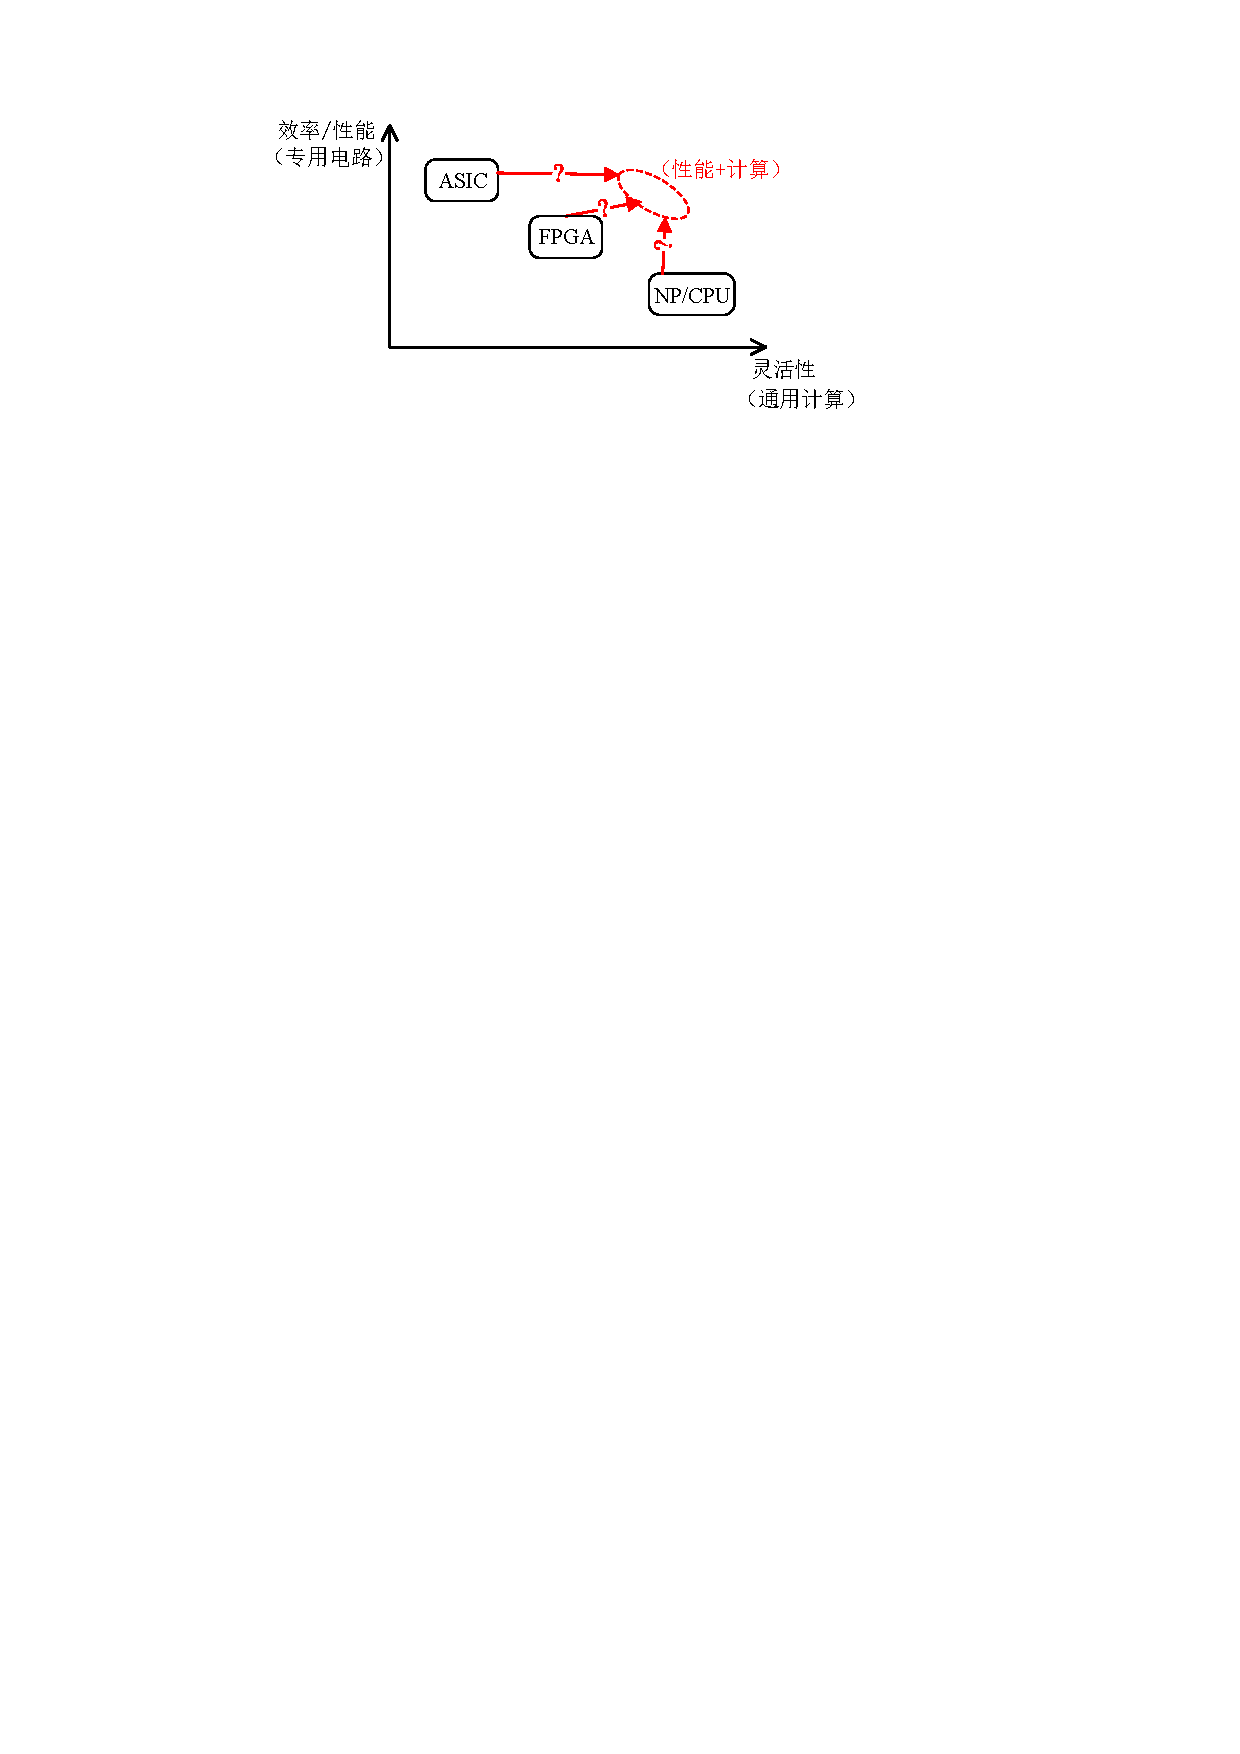
\includegraphics[scale=1]{generalprog.pdf}
	\caption{性能与灵活性如何更好的折中} \label{generalprog}
\end{figure}




\BiSubsection{领域内可编程性和可编程转发设备}{}%ipad笔记本

1)领域内可编程性
在不同的信息技术领域内有不同信息处理需求,从信息技术蓬勃发展的过去的几十年到现在,随着微电子行业的诞生,一直不断地涌现出各种类型基于某种专业硬件的处理器,往往这些设备都兼具有某种软件的可编程性。如图\ref{historyprocessors}所示,下面简要介绍历史各个类型可编程处理器。第一,中央处理器(CPU)。CPU解决的是通用类型的计算问题,工作生产生活中,人们往往会遇到各种各样的数学计算任务,使用CPU去辅助人们完成这类枯燥且量大的工作可以极高的提升社会生产效率。CPU采用冯诺依曼结构,是一种图灵机。它将处理通用计算任务抽象为控制-计算-存储模型。控制模块从存储器内读取程序指令和数据指令,并把他们按逻辑分配给计算模块。人们预先可以将需要处理的任务和数据编写到可重复擦写的存储器中,实现各种灵活的任务需求。操作人员就从繁琐的计算当中隔离开来,只需要去关注如何设计控制逻辑已经对应的需要计算的数据。第二图形处理器(GPU)。图形从本质上是一组二维矩阵数据,像素数据量一般都在百万级别。视频信号又是由一帧一帧的图像先后排列形成,导致处理图形的过程中产生大量的数据量。这些数据由CPU处理往往需要占用很长的处理时间,消耗大量的计算能力从而效率低下。GPU架构提出,图像处理没有先后依赖关系,处理器对于每一帧图像处理的方式完全一致,因而可以利用多CPU并行处理以达到加速目的。所以GPU就是众多微小的CPU的堆叠,同时增加了片上存储密度以应对并发的指令读取需求。第三,信号处理器(DSP)。与CPU类似,但DSP增加了专门为信号处理设计的指令集,使FFT运算更快速。DSP一般是数据地址与内存地址分开的双总线结构,支持灵活的编程。第四,神经网络处理器(NPU)。神经网络的训练过程需要进行大量的张量运算,适合于使用并行度高的处理器做运算,例如使用GPU。但在神经网络的计算中数据位宽往往比较低(8bits)如果使用通用处理器会有比较大的资源浪费,能源效率也比较低。随着AI技术发展,业界对算力的需求持续增高,研究人员专门为神经网络计算任务设计了一种专用处理芯片,TPU与GPU相比在同样能源消耗下,计算完成时间可缩短70倍左右\citeup{tpugoogle}。第五,协议无关交换架构(PISA)。网络包处理流程一般比较封闭,开发人员一般使用设备厂商固化好的网络设备进行数据包传输处理等。但由于网络功能应用环境的快速变化,研究人员发现固化的网络处理芯片无法满足增加新协议的需求,这严重制约了网络的创新。最近业界提出基于硬件的PISA模型,定义了可编程数据包处理的规范。它提出了开源的数据平面功能描述语言,为开发人员提供了可编程的包头描述能力,以及对应的包头信息抽取。在查找和匹配方法上,此类芯片使用多级查表法来实现任意的匹配和查找操作。

\begin{figure}[!ht]
	\centering
	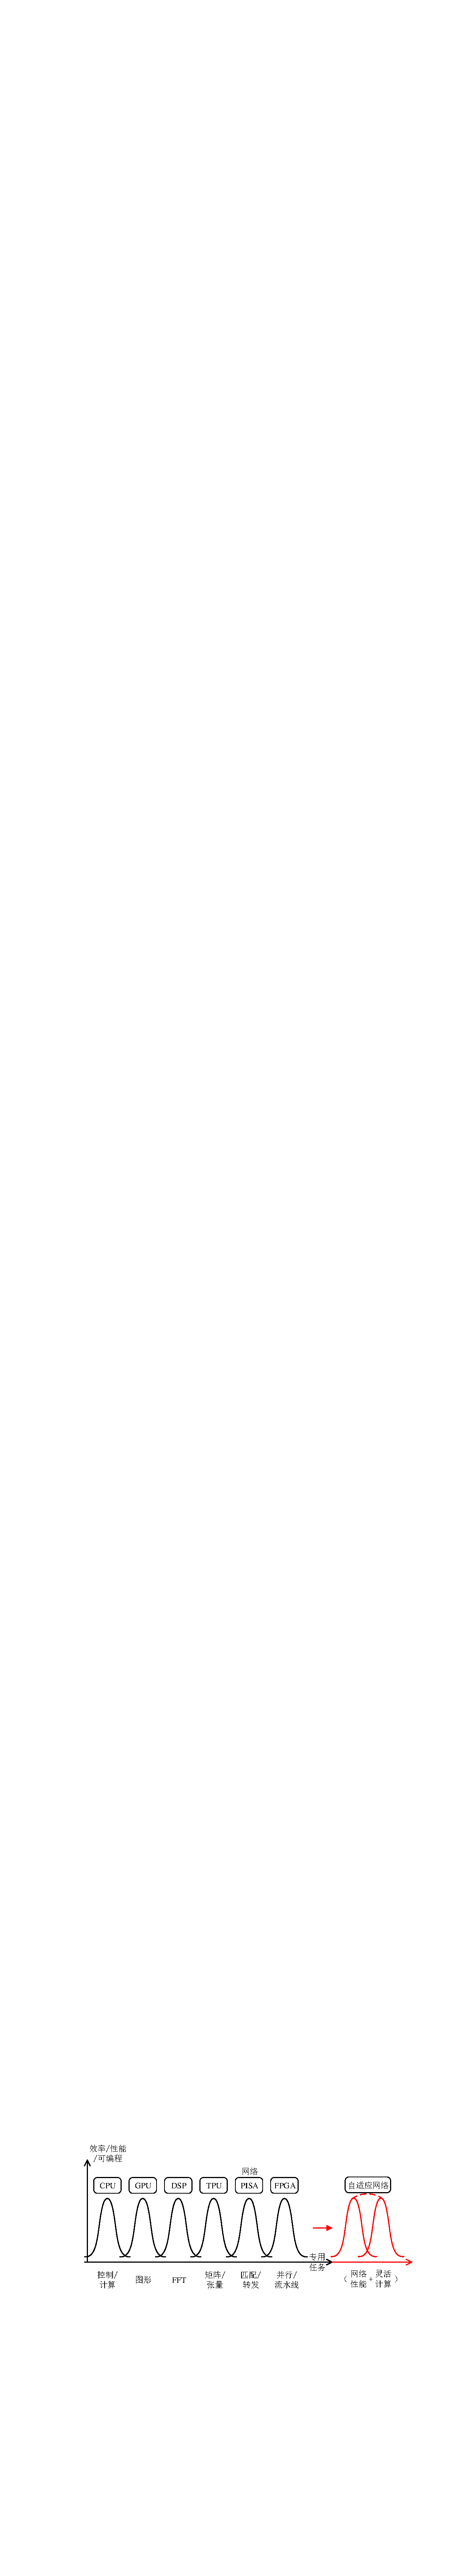
\includegraphics[scale=1]{historyprocessors.pdf}
	\caption{器件在不同的专用任务中性能和可编程性指标} \label{historyprocessors}
\end{figure}

在网络领域的可编程虽然较新,但已经引发业界很大的关注。不少工作都指出,可编程网络在超大规模数据中心网络、企业级交换网、网络内测量、负载均衡等领域都有广泛的实践以及优势。PISA有能力只使用单一器件就可支持种类繁多的网络功能,这种大的灵活性可为企业节约更换设备的成本,统一结构的数据平台也使操作人员维护复杂网络的成本降低。综上所述,网络可编程也已经作为可编程专用任务中的重要一分子,在未来值得持续投入研究。

%0)可编程的介绍
%1)如何引出可编程交换机
%2)详细介绍
2)可编程交换芯片架构

网络设备的最基本功能是解析数据包头,并对数据包头信息进行转发、丢弃、修改动作。最初的基于硬件的网络设备对于一个数据包包头定义是固化的,每当增加新协议字段,这种固化的网络设备都无法胜任新工作。但如果所有操作都由CPU处理,则性能十分低下,无法满足核心网、骨干网中性能的需求。后来人们针对处理数据包灵活性不足和性能问题对CPU进行架构优化,设计出采用辅助硬件流水线增强和多核并行方式的网络处理器。网络处理器拥有CPU般的灵活性,但由于本质还是基于CPU的指令循环操作,以及众核架构的内存、数据总线复杂度高数据搬运压力大,NP最终难以持续优化,目前业界顶级的基于NP的交换芯片性小于有1Tbps,这极大地限制了NP的使用范围。
新兴的基于ASIC流水线指令集的可编程处理器为NP的性能不足带来了一种解决思路(PISA)。

首先,需要解决基于ASIC的可编程包头解析器。交换机中的查找表必须查找固定协议字段,所以每个交换机都会包括一个包头解析器,它能够标识当前数据包包头的协议名称。
如图\ref{pktheader}所示,数据包是一组串行数据,从数据包的开始位置起,包头协议依次串行排列。每个协议段长度固定,每个协议末尾会有标识码标明下一个协议字段名称。本协议字段的长度一般都存储在协议字段内部。
包头中的协议字段是一种有向图关系,图的节点代表协议,向量字段代表转移关系。
一个包的包头不一定包含图中所有的节点,和对应关系,但当数据包到来时,包头所包含的协议只能是有向图中的唯一一种路径。一般使用有限状态机(FSM)就可以提取出包头内的所有协议字段。FSM内部存储完整的图关系,只要按照图对应关系来给包头不同字段打上协议名称标签即可。

\begin{figure}[htbp]
	\centering
	\begin{minipage}[t]{0.48\textwidth}
		\centering
		
\includegraphics[scale=1]{pktheader.pdf}
		\caption{数据包包头结构} \label{pktheader}
	\end{minipage}
	\begin{minipage}[t]{0.48\textwidth}
		\centering
		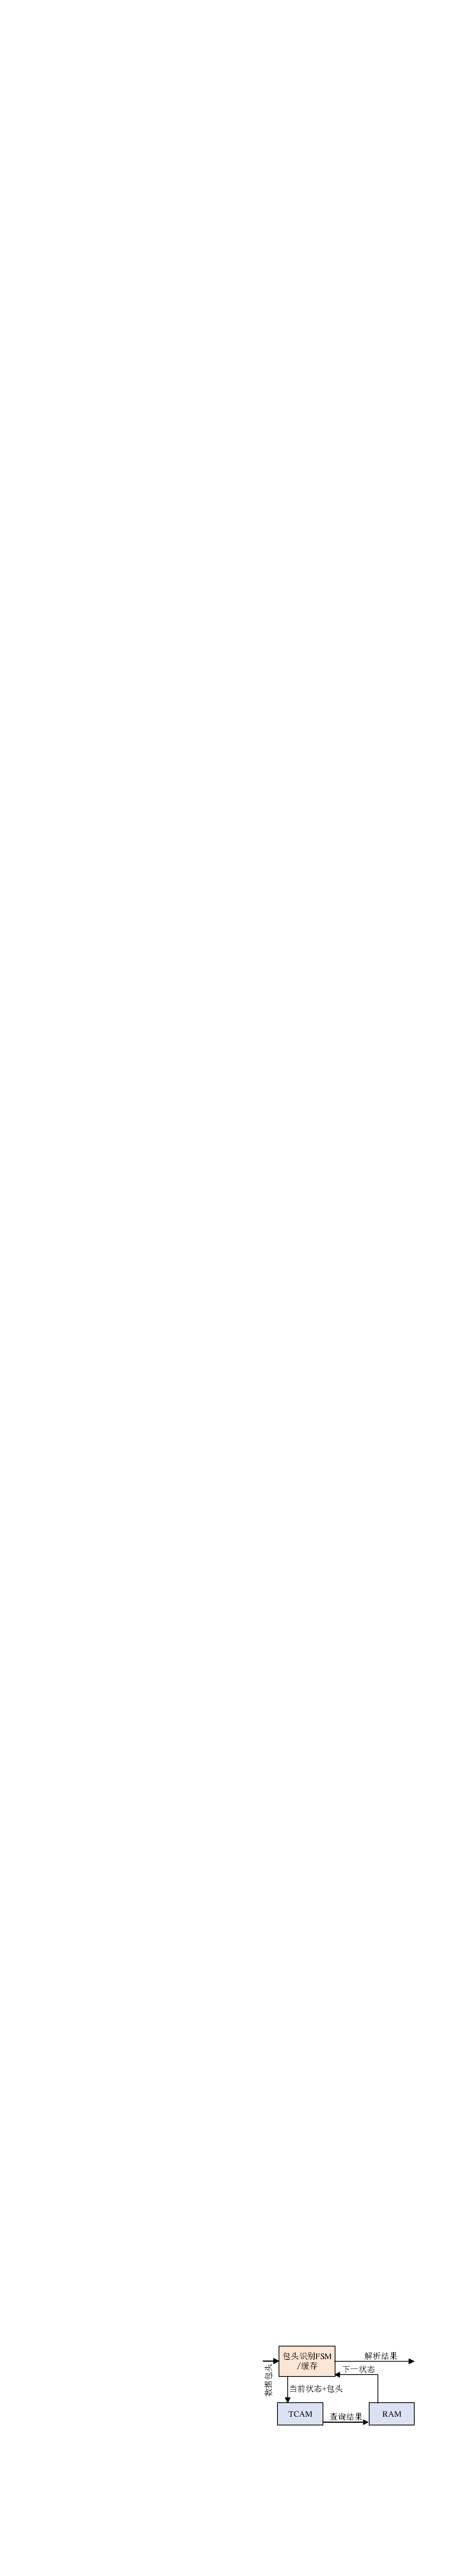
\includegraphics[scale=1]{progparser.pdf}
		\caption{基于ASIC的可编程包头协议解析器架构} \label{progparser}
	\end{minipage}
\end{figure}


可编程解析器须实现灵活可运行时配置的协议图。可编程解析器中的状态转移图可以通过状态查找表来实现。状态查找表可以由RAM 和/或 TCAM存储器组成,RAM是一种基于地址的内容访问存储器;CAM是一种基于内容的地址访问存储器。CAM中在不同地址存储有内容,当CAM接收到一个内容输入请求(key)时,可以并行搜索所有位置,并返回内容等于key的地址位置。TCAM则是在请求key中可以定义“不考虑”bit位,在判断二者内容是否相等时所有“不考虑”位都认为是相等的。如图\ref{progparser}所示,TCAM的key的宽度与一个完整的包头相等,在TCAM的一个表项中,存储着某一个协议的包头标识数据,这个数据的位置与真实数据包包头中此协议的位置相同,但是其他位置都属于“不考虑”bit位。因而只要包头可以匹配此TCAM表项,就代表包头中有这个协议。当然由于包头域是个有向图,在不同阶段所需要看的标识位置是不一样的。下一跳状态信息就存储在RAM中,得到新的状态后,电路再去查找TCAM,直到有向图走完。只要我们有足够宽的TCAM表,我们可以通过任意修改表中存储的状态图信息来实现运行时可编程的包头解析器。

第二,需要解决基于ASIC的可编程流表匹配。在传统交换机中,当数据包完成包头域的解析,交换机通过查询流表来得到数据包的执行指令。如图\ref{traditionalmatch}所示,处理每个协议的节点组成了协议有向图,节点一般可以抽象为“匹配--执行”的模式。由于包头协议状态转移图是固化的,所以交换机可操作的数据包的种类、数量也是固定的,其他数据包会被交换机当做未知类型而丢弃。在设计交换机之初,就需要根据各个协议字段不同位宽,不同流表匹配方法,制定固定深度的流表。因而目前固化交换机的数据处理核心都会设计异常复杂,需要适配各种有可能的协议,然而在某一个应用场景中只会存在其中一部分数据包类型,导致了很大能耗和经济的开销。



\begin{figure}[htbp]
	\centering
	\begin{minipage}[t]{0.48\textwidth}
		\centering
		
\includegraphics[scale=0.9]{traditionalmatch.pdf}
		\caption{传统交换机中的查找匹配过程} \label{traditionalmatch}
	\end{minipage}
	\begin{minipage}[t]{0.48\textwidth}
		\centering
		
\includegraphics[scale=0.90]{progmatch.pdf}%此图有更新 2020年7月4日15:28:26
		\caption{基于ASIC的可编程匹配模型} \label{progmatch}
	\end{minipage}
\end{figure}

可编程流表须实现灵活配置“查找--执行”逻辑结构。如图\ref{progmatch}所示,目前的设计思路,可编程匹配流水线由$N$个“物理块”(Phy\_Stage)串联而成,每个Phy\_Stage可以独立配置查找表的位宽、深度和类型。而且在每个Phy\_Stage中堆叠了所有类型的“执行器”(Action)模块,在运行时这些部件依次按流水线背靠背方式处理。选路器可以由多路复用器(MUX)或交叉开关(Cross\_Bar)组成。由于这些机构都可以被后期在线配置,在这样的流水线中一个1024bits的并行包头数据进入物理块后由第一个选路器(MUX)选出“待匹配域”送入所需的存储器接口,匹配之后的结果和包头域信息被第二个选路器(Cross\_Bar)送往所需的执行器中进行操作。最后执行器将新的域插入(修改/删除)包头内形成新包头。多个“物理块”可以先后呼应形成一个更复杂的“逻辑块”,最终通过运行时配置这些“物理块”可表达任意类型的协议有向图。


\BiSubsection{可编程数据平面的应用与问题}{}%已经有的成果和应用,展望我们工作的未来
% https://rg0now.github.io/prog_dataplane_reading_list/README.html#org37fc8b1 有很多应用和分类 %《可编程数据平面调研_说的还不错.pdf》
%《阿里巴巴》page11

%《软件定义网络带状态转发》 page22 openflow的不足
协议无关(PISA)处理器从诞生至今已经覆盖了广泛的网络应用场景:

1)替代传统网元(服务负载均衡\citeup{miao2017silkroad}、安全控制\citeup{lapolli2019offloading}、流量控制\citeup{yang2018elastic}、测量\citeup{kim2015band}),使云网络自身成为一个软硬任务分配均衡且可编程的系统。

2)增加网络随路专用功能,如键值查询(key-value store)\citeup{jin2017netcache}。旨利用网络高速以及可编程交换机特点,使特殊功能的性能大幅提升。

在此之外,也有很多特性是PISA架构无法实现的:

1)包头长度有限,目前数据平面可编程的流水线紧紧局限于处理宽度受限的包头。

2)非图灵完全,只有有限个数的固化的“执行器”。

3)没有讨论包调度问题。

4)无法对数据包进行可编程的带状态处理。

而这些问题目前被认为是因追求高性能而带来的设计折中\citeup{lec8rmtp4}。





\BiSection{网络资源优化}{} %已经有的成果和应用,展望我们工作的未来 周亚东 冷峻园的安全论文



\BiSubsection{软件定义网络安全通道机制}{}
%《软件定义网络关键技术及相关问题的研究》 page11

在前文提到过,软件定义网络(SDN)的诸多优势是由于网络结构分层带来的。SDN将控制平面抽离出来,形成对网络集中控制的局面。由于二者的远距传输,通信成本相对增大,主要体现在:第一,SDN强调网络的快速变化,然而控制器对数据平面的控制都依赖于容易成为瓶颈的安全通道。安全通道一般通信速率较低,而且控制信令传输延迟大。这与快速变化的网络结构成为矛盾。第二,成为中间瓶颈的安全通道容易承载来自内部、外部的大流量,而遭受攻击。

SDN的控制平面包括一个符合南向接口协议的网络操作系统,以及运行在其上的众多应用。SDN网络操作系统与下层数据平面通过安全通道相连。网络操作系统基本的任务是管理与配置。管理包括,发现交换机、发现拓扑、发现端口、故障测量等任务。配置包括,流表配置、执行集配置,组表以及限速表等配置。在支持数据平面可编程(PISA)的交换机中还会有包头解析器配置和数据平面逻辑块的配置。


\BiSubsection{数据平面流表资源与问题}{}
%ip1w 2.2.1
传统的表项查找方法都是基于SRAM的软件查找方法,共同特点是查找速度慢。线型查找法需要遍历表中的所有表项;二叉树查找法需要遍历树中大多数节点,而且查找速度受树的深度影响较大。
数据平面交换机设备为支持大量流快速查找,一般需要使用基于RAM/CAM的快速存储器。

查找表资源占比大。

%TCAM 面积 举例子 金额



\BiSection{本章小结}{}
核心思想是在不同时段,人们根据不同的现有即使做取舍从而满足技术需求。











































